\chapter{Introduction}%\label{chap:intro}
Research and development in the autonomous vehicle domain has been gaining momentum in the automotive industry over the last decade. Although the prospect of autonomous vehicles may still seem impossibly futuristic, technological advancements have paved the way to changing the way people view autonomous vehicles from impossible to inevitable. Every significant automaker is pursuing this technology field, eager to stay up-to-date and restructure its mindset to fit the rapidly growing innovative market.

\section{Motivation \& Problem definition}
Throughout history, humans have always attempted to automate mobility, starting with da Vinci's Self-Propelled Cart in the 1500s, going through the self-propelled Whitehead Torpedo in 1868, Mechanical Mike aircraft autopilot in 1933, Teetor Cruise Control in 1945, General Atomics MQ-1 Predator drone in 1995, and the infamous Tesla Autopilot in 2015.

Vehicles with at least basic autonomy can be found everywhere today. California, Michigan, Paris, London, Singapore and Beijing are the major cities to first host autonomous vehicles. Autonomous vehicles are expected to save hundreds of thousands of lives in the next few decades. On the other hand, it will devastate the auto industry and its associated infrastructure. However it is worth remembering that when automobiles first emerged, people called them "horseless carriages". A century later, it redefined how people move, and thus how they live. This cycle has restarted, and the term "driverless car" will soon seem as strange to the ear as "horseless carriage". The effect of autonomous vehicles on the society is unpredictable, however, it is obvious that a similar shift to the societal mindset is close.

The main motive behind the advancements in the field of self-driving cars is designing safer and easier means of transportation. This will in turn decrease the number of lives claimed by traffic accidents. The general mindset is directed to removing the Human from the driver’s seat by replacing sensory functions with Autonomous systems.

\subsection{Levels of Autonomy}
There are various levels of driving autonomy. Some basic autonomous functions are already in production and available in many vehicle on the road such as Adaptive Cruise Control and Lane Keep Assist. Additionally, there are sophisticated Active Safety systems that use complex sensors to provide functions such as Pre-safe (early) braking and Collision Avoidance. Generally, driving automation levels can be divided as follows:
\begin{figure}[ht]
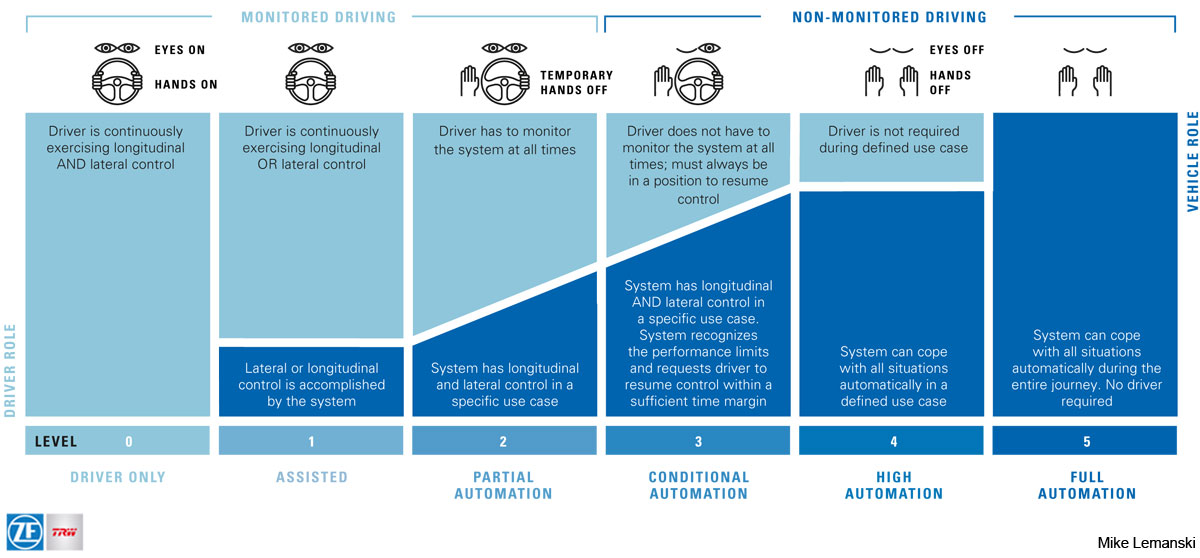
\includegraphics[trim={0 1.7cm 0 0},clip,width=\linewidth]{Figures/AutomatedDrivingLevels.jpg}
\caption{Autonomous Driving Levels}
\end{figure}
\subsubsection{Level 0 - No Automation}
All aspects of the dynamic driving task is the human driver's full-time responsibility.
\subsubsection{Level 1 - Driver Assistance}
The system can handle longitudinal or lateral control using information of the surrounding environment given that the driver handles all other aspects of the driving task.
\subsubsection{Level 2 - Partial Automation}
The system can handle both longitudinal and lateral control using information of the surrounding environment while the driver handles other aspects of driving such as global navigation in addition to monitoring the system and intervening whenever needed.
\subsubsection{Level 3 - Conditional Automation}
The system performs all aspects of the driving task within a certain situation, such as highway driving, with the expectation that the driver is monitoring and will intervene whenever needed.
\subsubsection{Level 4 - High Automation}
In a defined area and weather conditions, the system can perform all aspects of the driving task even if the driver does not respond appropriately to a system request or warning for human intervention.
\subsubsection{Level 5 - Full Automation}
The system can perform all aspects of the driving task in any environment and conditions in which a human is capable of driving. No Driver intervention is needed.
\section{Review of existing Products}
In today's market there are various existing products developed by Tier 1 Automotive suppliers such as Valeo, Bosch, Continental, etc. that support and contribute to complete an autonomous driving system. The most known of these systems are: 
\subsubsection{Lane Departure Warning}
LDW is not considered as a form of driving automation but rather an Advanced Driver Assistance System (ADAS). This is due to the fact that its main function is to warn the driver whenever the vehicle starts to depart from its current lane without prior signaling of a lane change. LDW is considered a passive-safety function, however, lane detection, which is a major component of this system, is a building block for having a unified environment perception that is essential for an autonomous vehicle.
\begin{figure}[h]
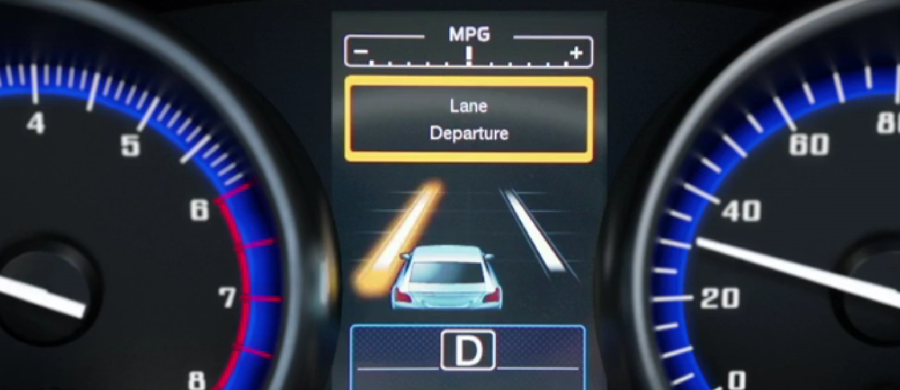
\includegraphics[width=0.6\linewidth]{Figures/LDW.png}
\centering
\caption{Lane Departure Warning}
\end{figure}
\subsubsection{Lane Keep Assist}
LKA is an active-safety function that compliments LDW with lateral vehicle control. Whenever the vehicle starts to depart from its current lane without prior signaling of a lane change, the systems intervenes with a brief steering input to correct the vehicle's trajectory.
\begin{figure}[h]
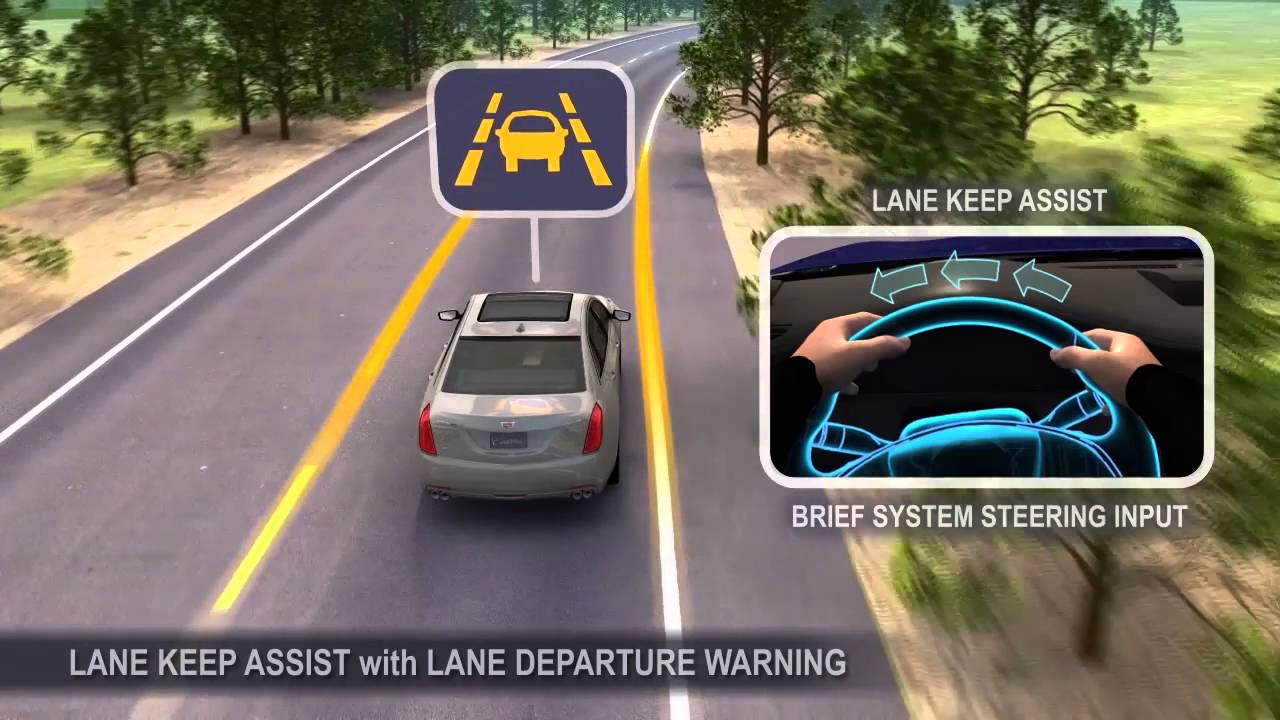
\includegraphics[trim={0 4cm 0 0},clip,width=0.6\linewidth]{Figures/LKA.jpg}
\centering
\caption{Lane Keep Assist}
\end{figure}
\subsubsection{Active Emergency Braking}
AEB aims at minimize front collisions. With the advancement in front-facing sensors, tracking vehicles is more efficiently done, which eases the task of automatic braking in case of a predicted collision.
\begin{figure}[h]
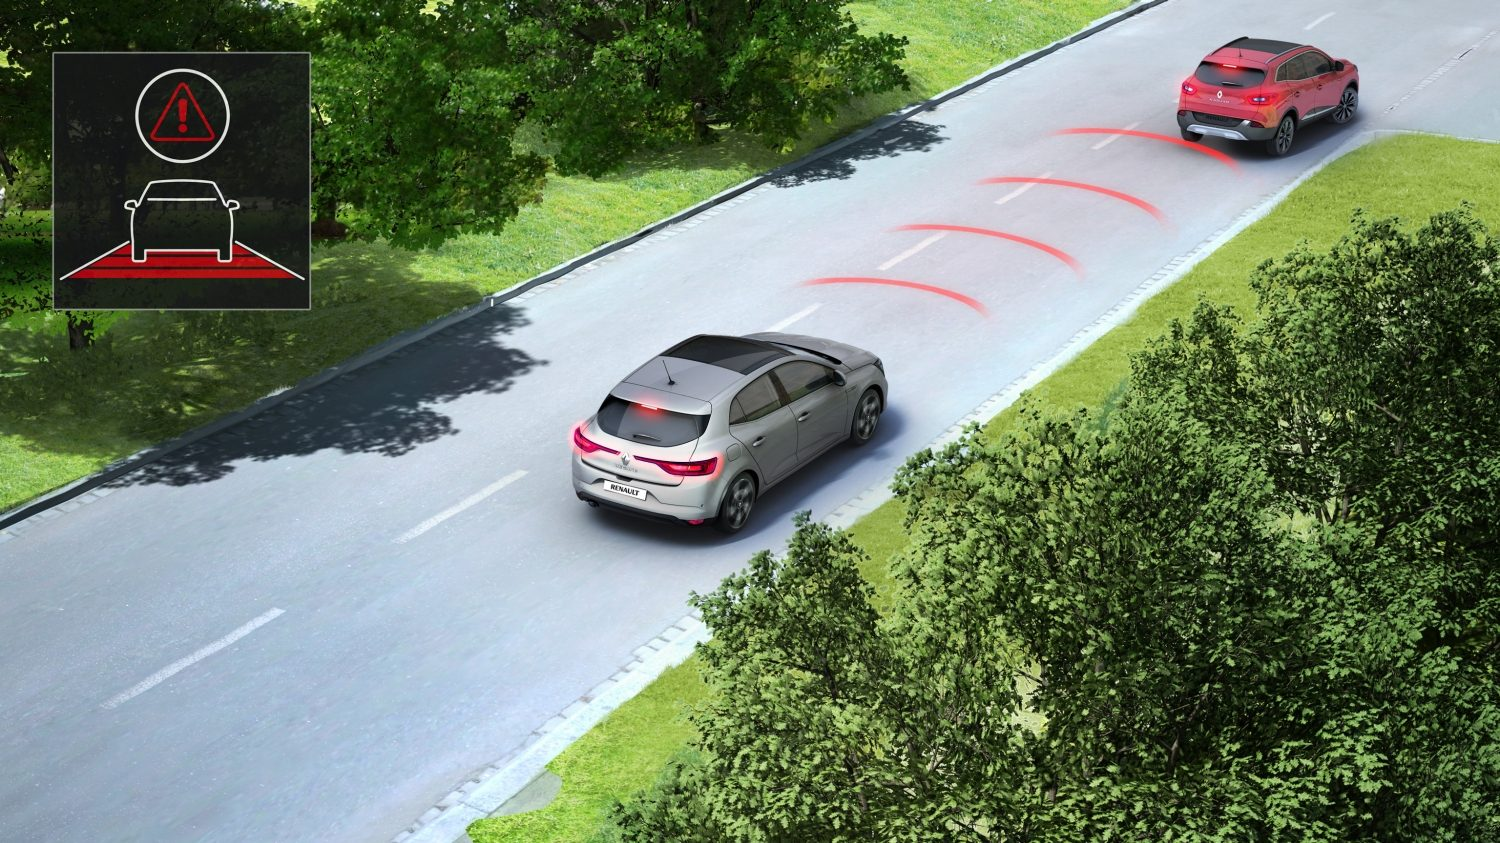
\includegraphics[trim={15cm 4cm 0 0},clip,width=0.5\linewidth]{Figures/AEB.jpg}
\centering
\caption{Active Emergency Brake \& Adaptive Cruise Control}
\end{figure}
\subsubsection{Adaptive Cruise Control}
ACC is the most used driving automation product. It aims at making highway driving experience more comfortable by taking over longitudinal control. The driver sets a desired distances to keep from the vehicle ahead, and a desired speed limit, and the system handles the throttle control to optimize those parameters.
\pagebreak